\documentclass[11pt]{article}
\usepackage[utf8]{inputenc} %%  codificoación: ñ, diéresis, etc..
\usepackage[T1]{fontenc} % Sin esto tendíamos que poner \'a
\usepackage[spanish]{babel} %% traducir comandos de LaTeX
\usepackage{xcolor} %% abanico amplio de colores
\usepackage{graphicx} % insertar gráficas o imagenes
\usepackage{float} % uso de imagenes flotantes
\usepackage{array} %para poder definir el ancho de las columnas en mi tabla de la siguiente manera: \begin{tabular}{|m{2cm}|m{5cm}}
\usepackage{booktabs} % dar mejor formato de tablas, uso de toprule, midrule,.... 
\usepackage{enumitem} % modificar listas numericas, alphanimericas, etc...
\usepackage{lipsum} % paquete para texto aleatorio
\usepackage{anyfontsize} %tamaño del texto
\usepackage{ragged2e} %para justificar un texto
\usepackage{hyperref} %para referenciar
\setlength{\columnsep}{30pt}


\hypersetup{
colorlinks = true, % si pones true elimina las cajas
linkcolor = rojo,
citecolor = azul 
}

%AMS ---> Formulas matemáticas
\usepackage{amsmath, 
            bm, 
            amsfonts, 
            amssymb}
\usepackage{geometry} % modificación de márgenes
\geometry{
    top = 0.8in,
    inner = 0.5in,
    outer = 0.5in,
    bottom = 0.9in,
}

\definecolor{blueM}{cmyk}{1.0,0.49,0.0,0.47}

\usepackage{fancyhdr} %modificación del encabezado y el pie de página
\pagestyle{fancy}

\fancyhead[c]{\small\color{azul} C. Rondan et. al} 
\fancyhead[r]{\color{gray} $|$ pag. N° \small\thepage}
\fancyhead[l]{}

\fancyfoot[c]{}
\fancyfoot[l]{}
\fancyfoot[r]{}

\renewcommand{\headrulewidth}{0pt}
\renewcommand{\footrulewidth}{0pt}

\definecolor{azul}{rgb}{0.11,0.38,0.65} %definir colores --> color{azul}
\definecolor{gris}{gray}{0.2}
\definecolor{rojo}{rgb}{0.65,0.12,0.06}


% Titlesec sirve para modificar el formato de los capítulos, secciones, subsecciones, etc..
\usepackage{titlesec}
\titleformat
{\section} %elegimos el nivel: captíulo, section, subsection ....
[hang]
{\Large\bf} % modifica las características que tendrá la siguiente línea de código
{\thesection.  } % Se puede poner algo antes del texto, por ejemplo la numeración 1.  o tal vez poner 'Capítulo' ...
{0pt} % Modifica el espacio izquierdo del texto, |INTRODUCCIÓN,  |    INTRODUCCIÓN 
{\Large} %modifica el texto, por ejemplo: que sea grande, cursiva, color azul, etc...s
[\vspace{-0.4cm}\rule{0.47\textwidth}{0.2pt}] 

\titleformat
{\subsection}
[hang]
{\normalsize\bf}
{}
{0pt}
{\itshape\large}
{}

\newcommand{\Color}[1]{\hypersetup{linkcolor=#1}\color{#1}} % lo usaremos para chancar los colores y priorizar la coniguración de lo hipervinculos

\usepackage{tocloft}
%%%%%%%%%% ESPACIO ENTRE INDICE, INDICE DE FIGURAS E INDICE DE CUADROS
\setlength{\cftbeforetoctitleskip}{.5cm} % espacio antes de la tabla de TOC
\setlength{\cftaftertoctitleskip}{0cm} % espacio despues del TOC

\setlength{\cftbeforeloftitleskip}{.5cm} % espacio antes de la tabla de LOF
\setlength{\cftafterloftitleskip}{0cm} % espacio despues del LOC

\setlength{\cftbeforelottitleskip}{.5cm} % espacio antes de la tabla de LOF
\setlength{\cftafterlottitleskip}{0cm} % espacio despues del LOC

%%%%%%%%%% CONFIGURACIÓN DE LETRA DE INDICE, INDICE DE FIGURAS Y,..
\renewcommand{\cfttoctitlefont}{\bf\color{azul}\hfil\Large\sffamily} % configuración del titulo del TOC
% cambiar lo que está en {} por toc, lof o lot---> \cft{toc}titlefont
\renewcommand{\cftloftitlefont}{\bf\color{azul}\hfil\Large\sffamily} 
\renewcommand{\cftlottitlefont}{\bf\color{azul}\hfil\Large\sffamily} 


%%%%%%%%%% TIPO DE LETRA DE SECCIÓN, SUBSECCIÓN, FIGURA, TABLA
%%% Modificar texto, incluye tamaño, color, tipo de texto ,etc...
\renewcommand{\cftsecfont}{\bf\Color{black}} %modificar el texto TOC de section
\renewcommand{\cftsubsecfont}{\Color{gris}}  %modificar el texto TOC de subsection

\renewcommand\cftfigfont{\bf\Color{black}}

\renewcommand\cfttabfont{\bf\Color{black}}

%%%%%%%%%%% CONFIGURACIÓN DE LA NUMERACIÓN
\renewcommand{\cftsecpagefont}{\color{gris}} % modificar el color de la numeración de la TOC en section
\renewcommand{\cftsubsecpagefont}{\color{gris}} %modificar el color de la numeración de la TOC en subsection

\renewcommand{\cftfigpagefont}{\color{gris}}

\renewcommand{\cfttabpagefont}{\color{gris}}


%%%%%%%%%%%% 
\setlength{\cftbeforesecskip}{0.15cm} %espacio antes de cada sección (en la tabla)
\setlength{\cftbeforesubsecskip}{0.15cm} %espacio antes de cada subsección (en la tabla)
\setlength{\cftbeforesubsubsecskip}{0.15cm}%espacio antes de cada subsubsección 

\setlength{\cftbeforefigskip}{0.15cm}

\setlength{\cftbeforetabskip}{0.15cm}

%%%%%%%%%%% AÑADIR SECCION, SUBSECCION, FIGURA, TABLA EN INDICE

\renewcommand\cftsecpresnum{\sffamily Sección }
\setlength{\cftsecnumwidth}{2.0cm} %distancia de las palabras con la numeración (section)
\renewcommand\cftsubsecpresnum{\sffamily Sub sección }
\setlength{\cftsubsecnumwidth}{2.5cm} %distancia de la letra al numero 1. (espacio) nombre

\renewcommand\cftfigpresnum{\sffamily Figura }
\setlength{\cftfignumwidth}{1.8cm}

\renewcommand\cfttabpresnum{\sffamily Figura }
\setlength{\cfttabnumwidth}{1.8cm}


%%%%%%%%%%%%%% PUNTOS EN EL INDICE , FIGURAS Y EN TABLAS
\renewcommand\cftsecleader{\cftdotfill{2}}
\renewcommand\cftsubsecleader{\cftdotfill{5}}

\renewcommand\cftfigleader{\cftdotfill{5}}

\renewcommand\cfttableader{\cftdotfill{5}}

%%%%%%%%%%%%%%%%




\addto\captionsspanish{\renewcommand{\figurename}{\small\sffamily \textcolor{azul}{\bfseries Fig. N°}}}  %cambia formato del caption   % le quité \itshape
\addto\captionsspanish{\renewcommand{\tablename}{\small\sffamily \textcolor{azul}{\bfseries Tabla N°}}}  %cambia formato del caption



\usepackage[square,numbers]{natbib} %[square,numbers] , round
\bibliographystyle{unsrtnat} %abbrvnat

\begin{document}

\begin{center}
    \begin{spacing}{2}
    {\bf\fontsize{19}{21}\selectfont\color{azul} Aplicación de la metodología QM - CRISP DM
para la reducción del desperdicio de frutas en el
mercado modelo la Victoria}
    \end{spacing}
\vspace{1mm}
    {\bf (Application of the QM - CRISP DM methodology to reduce fruit waste in the La Victoria model market)}
    
    
    \vspace{2.5mm}
    {\small Carlos Rondan Poma, Universidad Nacional de Ingeniería, Perú\\
Enrique Elera García, Universidad Nacional de Ingeniería, Perú\\
Johana Surco Huancas, Universidad Nacional de Ingeniería, Perú\\
José Gutierrez Saravia, Universidad Nacional de Ingeniería, Perú\\
Luz León Churquipa, Universidad Nacional de Ingeniería, Perú}
    
\end{center}

\begin{spacing}{0.95}
\footnotesize\noindent\itshape Resumen: Perú es el octavo país que produce y genera más desperdicios de plátanos, desperdicio equivalente a
37 millones de dólares a nivel nacional; todo esto sin mencionar los desperdicio que generan las demás frutas.
En este proyecto proponemos aplicar la metodología QM-CRISP DM para determinar las causas de desperdicio
en la cadena de valor del mercado modelo La Victoria. En consecuencia, nuestra propuesta de mejora ataca dos
frentes importantes, el primero es la aplicación de la metodología 5 s en el mercado mayorista y el segundo es
la aplicación de inteligencia artificial para la detección y clasificación del nivel de calidad de los plátanos y
estimación del tiempo de vida útil.
\vspace{-0.2cm}
\begin{center}
    Palabras Clave: Desperdicio de frutas, DMAIC, CRISP-DM, metodología 5s, Aprendizaje profundo
\end{center}
\end{spacing}

\begin{spacing}{0.95}
\footnotesize\noindent\itshape Resumen: Perú es el octavo país que produce y genera más desperdicios de plátanos, desperdicio equivalente a
37 millones de dólares a nivel nacional; todo esto sin mencionar los desperdicio que generan las demás frutas.
En este proyecto proponemos aplicar la metodología QM-CRISP DM para determinar las causas de desperdicio
en la cadena de valor del mercado modelo La Victoria. En consecuencia, nuestra propuesta de mejora ataca dos
frentes importantes, el primero es la aplicación de la metodología 5 s en el mercado mayorista y el segundo es
la aplicación de inteligencia artificial para la detección y clasificación del nivel de calidad de los plátanos y
estimación del tiempo de vida útil.
\vspace{-0.2cm}
\begin{center}
    Palabras Clave: Desperdicio de frutas, DMAIC, CRISP-DM, metodología 5s, Aprendizaje profundo
\end{center}
\end{spacing}
\tableofcontents
\section[Introducción]{Introducción}

\lipsum[1-3]
\lista{
    \item \lipsum[1]
    \item \lipsum[1]
}


\lipsum[1]

\subsection{Planteamiento del problema}

\lipsum[1-3]

\begin{table}[h!]
    \centering
    \begin{tabular}{rrr}
\toprule
 floor\_area &  year\_built &  nueva variable \\
\midrule
    61242.0 &      1942.0 &     118931964.0 \\
   274000.0 &      1955.0 &     535670000.0 \\
   280025.0 &      1951.0 &     546328775.0 \\
    55325.0 &      1980.0 &     109543500.0 \\
    66000.0 &      1985.0 &     131010000.0 \\
   119900.0 &      1956.0 &     234524400.0 \\
    91367.0 &      1982.0 &     181089394.0 \\
    50422.0 &      1947.0 &      98171634.0 \\
   122020.0 &      1929.0 &     235376580.0 \\
   102612.0 &      1979.0 &     203069148.0 \\
    65998.0 &      1979.0 &     130610042.0 \\
   100000.0 &      1927.0 &     192700000.0 \\
   128320.0 &      1960.0 &     251507200.0 \\
   616793.0 &      1955.0 &    1205830315.0 \\
    53000.0 &      1924.0 &     101972000.0 \\
    90045.0 &         NaN &             NaN \\
    74055.0 &      1949.0 &     144333195.0 \\
   128800.0 &      1926.0 &     248068800.0 \\
    91619.0 &      1914.0 &     175358766.0 \\
    53280.0 &      1973.0 &     105121440.0 \\
   217710.0 &      1900.0 &     413649000.0 \\
    68538.0 &      1913.0 &     131113194.0 \\
    90669.0 &      1962.0 &     177892578.0 \\
\bottomrule
\end{tabular}
    \caption{Consumo energético}
    \label{tab:my_label}
\end{table}

\begin{figure}[h!]
    \centering
    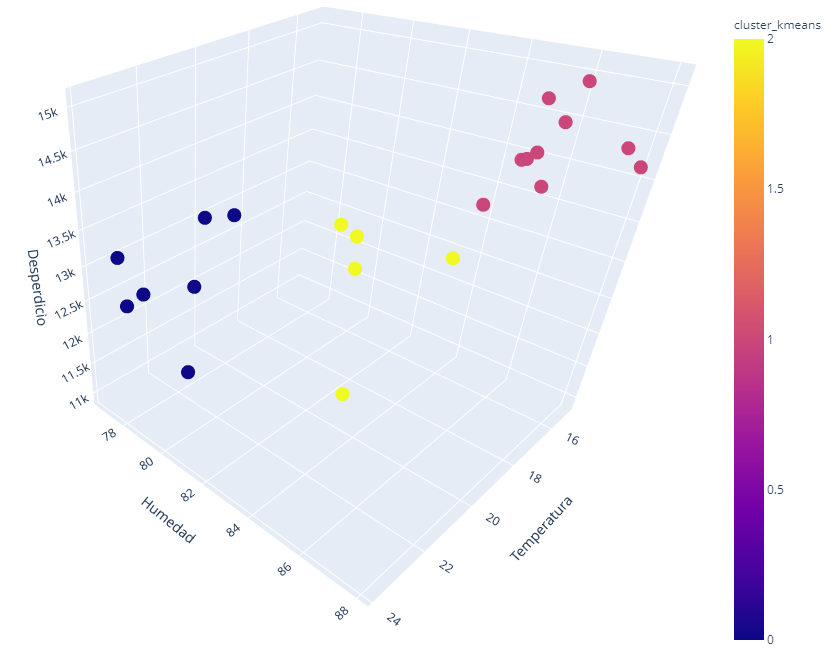
\includegraphics[width = 11cm]{figuras/cluster_3D.PNG}]
    \caption{Imagen de un cluster}
\end{figure}

\figura{5cm}{cluster_3D}{Ssoy una imagen de cluster\label{imagen_3D}}
\newpage
La imagen usando un algoritmo de machine learining del tipo K mean (ver figura \ref{imagen_3D})

\section[ANTECEDENTES]{Antecedentes}
\lista{
    \item \lipsum[1]
    \item \lipsum[1]
}
\input{metodologia}
\input{resultados}
\input{conclusiones}


\end{document}
